\documentclass[a4paper]{book}
\usepackage{graphicx}
\usepackage{caption}
\usepackage{subcaption}
\usepackage[brazil]{babel}
\usepackage[utf8]{inputenc}
\usepackage{fullpage}
%
%
% DICAS GERAIS:
%	* LEIA O TEXTO ESCRITO
%	* ATIVE OS REVISORES GRAMATICAIS
%	* PREOCUPE-SE INICIALMENTE COM O CONTEÚDO, DEIXE PARA DEPOIS A ESTÉTICA E A EDIÇÃO
%	* SEJA OBJETIVO E EVITE REDUNDÂNCIA
%	* NUMERE AS EQUAÇÕES
%	* PARA AS LISTAS, TENTE USAR AS FUNÇÕES AUTOMÁTICAS DOS EDITORES
%	* IDEM PARA AS REFERÊNCIAS
%
%
\begin{document}

\chapter{Introdução} \label{chap:intro}

%% Histórico

	Ao longo dos últimos quarenta anos, com a difusão de tecnologias eletrônicas modernas, a palavra ``digital'' tem se tornado cada vez mais lugar comum. Ao longo desse período, a tecnologia baseada em máquinas de cálculo automatizado que ocupavam prédios inteiros e eram operadas por poucos (para fins restritos) foi permeando nossa cultura global e ganhando destaque em vários campos do conhecimento e da vida humanas. Com o passar do tempo, as suas aplicações foram ganhando horizontes, os computadores passaram a ser pessoais e cada vez mais amplamente utilizados, contudo, ainda tinham aplicações específicas em ambientes de pesquisa e para atividades profissionais, e eram restritos a mesas e ambientes reservados. Em paralelo, a indústria de jogos eletrônicos começa a florescer, se fazendo presente nas residências através de seus consoles. Todos aproveitavam a evolução tecnológica apresentada pelo advento dos transistores e microprocessadores.

	Adiante mais alguns anos, e a internet aparece, os microprocessadores estão mais ``micro'' e mais ``processadores'', os consoles de video-game mais elaborados e seus clientes cada vez mais exigentes. Os microprocessadores vão transitando de máquinas estáticas para aplicações móveis: celulares e câmeras digitais (para foto e vídeo) tornam-se quase onipresentes. Mídias digitais tornam-se tão importantes quanto protocolos de comunicação, redes sociais movimentam a opinião pública e servem de plataforma a revoluções ~\cite{revoltaEgito}. Muitos cidadãos globais têm contas em várias redes sociais e máquinas portáteis em seus bolsos, prontas a fazer um vídeo ou uma foto e postá-los para apreciação popular. Ao que se faz possível, com alguns poucos cliques e nenhum custo com passagem ou hospedagem, termos acesso à realidade atualizada de diversas partes do globo, em todos os idiomas possíveis, a qualquer hora.

	O volume de dados gerado é tão grande que plataformas como o Flickr (da americana Yahoo) abrigava, em 2011, mais de seis bilhões de imagens digitais ~\cite{flickr6bi}, e o crescimento estimado para o crescimento de seu banco de imagens nos anos seguintes foi de um bilhão por ano --- e essa é apenas uma de várias plataformas de hospedagem de publicação de mídias ~\cite{500px} \cite{instagram}. Outro exemplo, para publicação de vídeos, é o Youtube, onde seus mais de um milhão de usuários únicos assitem mais de seis bilhões de horas de vídeo por mês. Outras plataformas de publicação de vídeo também têm números expressivos, como o caso do Vimeo, com mais de 200 \emph{petabytes} de vídeos executados em 2012 ~\cite{vimeo}. Além de serviços de hospedagem de conteúdo disponíveis publicamente, mais recentemente surgiram serviços de \emph{streamming} de filmes e séries, como o Netflix, já com mais de 40 milhões de usuários em 41 países, disponibilizando mais de um bilhão de horas de vídeo~\cite{netflix}.

	Esses números representam um desafio para a indústria, que se responsabiliza por receber, armazenar e distribuir esses dados sob demanda, para todo o globo.

	Voltemos um pouco à história de alguns parágrafos acima. Outra entidade que acompanha esse desenvolvimento, e que o antecede em algumas décadas é a televisão, cujo pai aclamado é Philo Farnsworth, entre tantos outros engenheiros e contribuições~\cite{tvhist}. Desde 1929 existe programação regular para TV sendo projetada no espaço, proveniente de ambos os lados do Atlântico (os Estados Unidos e o Reino Unido começaram a produzir programação regularmente na segunda metade de 1929)~\cite{tvhist}. 

	Com o nascimento dessa tecnologia, começou-se a discutir a necessidade de avaliar a qualidade da imagem recebida em aparelhos de TV, e artigos como ``\emph{ Television images: an analysis of their essential qualities}'', publicado por Jesty e Wintch, em 1937\cite{Jesty1937}, aparecem. Winch, começa seu artigo de 1953~\cite{Winch1953} com a afirmação (em tradução livre) ``a adição de cores à televisão traz muitos novos problemas a um assunto já complexo". E já em 1940, Peter Goldmark e John Dyer ~\cite{Goldmark1940} apresentam quais características são mais importantes ao determinar-se a qualidade de uma imagem (para TV): definição, faixa de contraste, ângulo de visualização (\textbf{gradation?}), brilho, efeitos da frequência de varredura (\emph{flickering}) , distorção geométrica, tamanho, cor e ruído. Algumas dessas características viriam a se tornar objetos de estudo da AQI nos anos vindouros, bem como algumas delas seriam bases para o cálculo de métricas de qualidade de imagem (fotografia e vídeo) --- falaremos de algumas delas nesse trabalho.

	Dado que a parte visual de um vídeo é constituída de imagens paradas em sequência, a avaliação da qualidade de vídeo e de imagem andam entrelaçadas desde o início. Tanto o é, que a International Telecommunications Union --- ITU (União Internacional de Telecomunicações, tradução livre) não faz distinção em seus documentos de padronização de qualidade entre vídeo e imagem~\cite{itut2004}; e seu grupo especializado para esse fim é chamado \emph{Video Quality Experts Group} (VQEG, Grupo de Peritos em Qualidade de Vídeo, tradução livre). Em ~\cite{itut2004}, encontramos recomendações para avaliação de qualidade de vídeo que podem ser também apliadas a imagens. Nesse trabalho seguiremos essas recomendações.

	Vê-se que, com tanta demanda por imagem e vídeo, e tráfego destes, é necessário que se encontre uma forma de armazená-los eficientemente, acessá-los confiávelmente e garantir que o usuário final terá a qualidade esperada, ainda que compressões e descarte de informações sejam necessários. Enquanto alguém preocupado com a compressão de uma imagem se perguntaria ``qual a menor quantidade de informação necessária para que se mantenha a completude da mensagem (no nosso caso, imagem)?'', um pesquisador atual de AQI se pergunta: ``como aferir a qualidade de uma imagem digital? Dado que a necessidade de reduzir a quantidade de informação é premente, o que garante qualidade percebida?''

	Essa é uma pergunta razoávelmente complexa, já que envolve conceitos abstratos e subjetivos. Uma boa imagem para uma aplicação não o é, necessáriamente para outra. Um exemplo simples é a aquisição de vídeos de segurança em comparação com a aquisição de vídeo para entretenimento. No primeiro caso, a qualidade mínima e suficiente é aquela que garante a identificação de um possível infrator; na segunda as exigências são mais altas (ninguém sentiria prazer em assistir toda a saga de Star Wars em preto e branco e com todo o ruído e baixa resolução que são aceitáveis para câmeras de segurança). É claro, não se pode deixar de lado as considerações sobre custo-benefício: no primeiro caso a resolução tem que ser mínima e suficiente para a identificação de um eventual infrator, mas também tem que ocupar pouco espaço em disco, já que câmeras de segurança, em sua maioria, funcionam continuamente. Quanto a Star Wars, o tamanho é fixo, uma vez terminada a edição; e a garantia da qualidade do produto final significa aumento de lucros em bilheterias pelo mundo afora.

	Tradicionalmente, existem duas formas de se construir algoritmos de AQI que possam determinar automaticamente a adequação de uma imagem para consumo humano~\cite{Chandler2013}: algoritmos baseados no sistema visual humano (SVH) e algoritmos baseados em sessões de avaliação.

	Algoritmos baseados em SVH levam em consideração a física de todo um sistema biológico, bem como a parte psicológica da percepção visual. Esse trabalho não tratará desse tipo de algoritmo e o leitor é direcionado aos trabalhos de ~\cite{Takemura2002} e ~\cite{Winkler-2005-Wiley}\ para maiores informações. 
	
	A segunda abordagem, que será alvo de estudo nesse trabalho, não aborda a psicofísica e se concentra em características da imagem que sejam relevantes. Para obter esses dados, sessões de avaliação são organizadas, onde pessoas são questionadas a respeito da qualidade de um conjunto de imagens. Após coletados os dados, o pesquisador tenta produzir um modelo que tenha como saída uma nota aproximada daquela dada pelos entrevistados. Obviamente, quanto menor o erro entre o sistema modelado e a avalição subjetiva dos indivíduos entrevistados, melhor o modelo.

	Aqui trabalharemos com duas bases de imagens distintas, proveniente de grupos de pesquisa independentes, que coletaram avaliação para as imagens constantes em suas bases de forma muito similar. Trataremos dessa similaridade, e eventual diferença no cap /ref{}. Ambos os grupos de pesquisa, seguem o que é de praxe na área, e tratam seus procedimentos de avaliação estatisticamente com muito critério, segundo as recomendações do ITU e o usualmente praticado na área.

	O questionamento que propomos é justamente sobre as ferramentas estatísticas utilizadas no tratamento desses dados e na validação das métricas em uso. Entendemos que, dada a natureza dos experimentos de avaliação e a forma como as notas são atribuídas às imagens, ferramentas de estatística em classes seriam mais adequadas para a análise dos resultados, e consequente pondereção de qualidade das métricas desenvolvidas sobre esses dados. Atualmente, as ferramentas estatísticas utilizadas nesse contexto são as mesmas utilizadas para tratar dados intrinsecamente não-categóricos.

	

	Esse documento está estruturado em X partes, resumidamente descritas abaixo:

\begin{description}
\item{\textbf{Introdução:} } breve histórico da área de Avaliação de Qualidade de Imagem, breve descrição do objetivo do trabalho e descrição suscinta das ferramentas utilizadas
\item{\textbf{Antecedentes:} } detalhamos melhor nossa proposta de trabalho, situamos o leitor quanto às abordagens estatísticas utilizadas na área e nossas ferramentas de comparação.
\item{\textbf{Procedimentos Experimentais:} } apresentamos as bases de imagem que serão utilizadas, os métodos utilizados e resultados preliminares de comparação com a literatura existente.
\item{\textbf{Análise Categórica:} } aprofundamos a explicação das ferramentas utilizadas, aplicamos essas ferramentas aos dados apresentados nos capítulos anteriores e efetuamos comparações de sua validade.
\item{\textbf{Conclusão:} } considerações finais sobre o trabalho e possíveis caminhos a serem tomados a partir das conclusões apresentadas.
\item{\textbf{Referências:} } lista de documentos que serviram de base para a produção desta obra.
\end{description}
 % Introdução
% Qual o problema a ser resolvido pelo trabalho?
% Por que ele é importante (contexto)?
% Quais as contribuições do trabalho para a solução do Problema?
% Os resultados/contribuições devem ser enumerados e descritos de forma sucinta (1 parágrafo por resultado, por exemplo). O TCC deve ser organizado em 
% torno destes resultados, portanto, devem ser muito bem identificados no início.
% Guia de leitura do TCC. Apresenta a lógica do TCC e indica o que vai ser encontrado em cada capítulo. É importante que o leitor saiba o que vai
% encontrar no TCC.
%

%\showthe\columnwidth
\chapter{Preâmbulo Teórico}

Para que possamos fazer uma análise comparativa entre duas estratégias estatísticas, temos que, antes, entender suas diferenças e similaridades, bem como as características dos dados com os quais estamos lidando.

Assim, este capítulo será dividido em três grandes seções, uma destinada à apresentação das bases de imagens utilizadas, outra destinada à apresentaçãodas métricas de qualidade de imagem e as utilizadas nesse trabalho; a última apresentando informações sobre ferramentas estatísticas.

\section{Avaliação de Qualidade de Imagens}

Como dito na \nameref{chap:intro}, os atuais usos de imagens e vídeos digitais têm sua abrangência amplificada, na medida em que novos serviços surgem no mercado --- e que mais usuários utilizam esses serviços. Isso, como dito, se torna um desafio pra indústria, que precisa encontrar formas cada vez mais econômicas e eficientes de entregar seus produtos (mídias digitais) utilizando a infra-estrutura de comunicação existente e com o mínimo custo computacional e de armazenamento.

Para resolver problemas de armazenamento e tráfego, algoritmos de compressão foram desenvolvidos e são utilizados corriqueiramente. Padrões de compressão, como o JPEG e MPEG (imagem e vídeo, respectivamente), são muito frequentemente utilizados no tráfego de dados via internet. Esses algoritmos podem ser divididos em duas categorias: a dos ``com perdas'' (\emph{lossy}) e a dos ``sem perdas'' (\emph{lossless}).

Exemplos de algoritmos \emph{lossless} para imagens são PNG e TIFF. ``Sem perdas'' significa que, uma vez descompactas, as imagens resultantes guardam as mesmas características das images originais --- o mesmo volume de dados dentro da mesma conformação espacial. Exemplos de algoritmos \emph{lossless}, que consideram a perda de informação como razoável e atingem taxas de compressão mais elevadas, são os já citados JPEG e MPEG.

A nós interessam considerações sobre os métodos de compressão com perdas, já que eles são capazes de economizar mais banda da rede de comunicação e otimizar ainda mais o armazenamento, em relação aos métodos sem perdas. Estabelece-se então uma relação de compromisso entre compactação e qualidade. Qual o mínimo de informação para que, aferindo economia dos custos de armazenamento e transmissão, mantenha-se a mesma qualidade percebida no produto final? Nesse contexto se situa o campo de pesquisa em qualidade de imagem. E como aferir essa qualidade? Atualmente, encontra-se duas formas distintas e dependentes: os métodos subjetivo e objetivo de aferição de qualidade visual.

\subsection{Avaliação Subjetiva de Qualidade}\label{sec:avSub}

	O método subjetivo ainda é o mais confiável, pois se baseia na aferição de qualidade a partir de observações humanas: à pessoas são apresentadas imagens, cujas qualidades são aferidas e anotadas. Esse método, contudo, apresenta algumas restrições e a primeira delas é a econômica. Para que a aferição seja feita por seres humanos é necessário, em geral, que esses sujeitos sejam pagos para tal tarefa, implicando também em espaço próprio para esse tipo de atividade, e portanto, mais custos. O segundo grande custo é o tempo: aferições humanas dependem de logística e tempo para o processamento dos dados obtidos.

	Outra questão é a da validade das medidas. Para que se tenha uma opinião considerada estatisticamente relevante para uma população, é necessário um grande número de sessões de avaliação, com uma gama de indivíduos bastante diversa --- idealmente, diversa a ponto de representar uniformemente todas as variâncias da população em questão. Essa consideração reforça as restrições de tempo e de custo financeiro. Esse tipo de avaliação é raramente executada com indivíduos ou imagens suficientes para que se possa fazer inferências a respeito do público em geral, apesar de o ITU recomendar no mínimo 15 (quinze) sujeitos distintos em cada sessão de avaliação~\cite[p.08]{itur2012}. Como será visto na seção seguinte (\autoref{sec:imdb}), as bases com as quais trabalhamos, largamente conhecidas e exploradas nas literaturas da área, tem poucas imagens e ainda menos avaliações (ainda que dentro dos padrões recomendados pelo ITU). Portanto, inferências para uma população são inviáveis a partir dessas observações --- que servem apenas para fins acadêmicos.

Problemas que podem ser encontrados em estudos estatísticos são os chamados ``\emph{bias}'', que podem ser inseridos em um estudo a partir da amostragem indevida da população para participação nos testes~\cite{boslaugh2008}, ainda na fase de design de tais testes. Esse tipo de consideração deve ser feita sobre as imagens que analisamos, já que estudos demonstram que ``experts'' na área de qualidade visual tentem a ser mais criteriosos em suas avaliações de qualidade; principalmente por já saberem o que procurar, no que tange erros e distribuição espacial destes~\cite[p.08]{itur2012}. Apesar de a Toyama alegar que seus sujeitos são não-peritos, ela também alega que são estudantes de nível superior, e que, portanto, não representam bem a população de possíveis consumidores de imagens, que podem ter não só níveis diversos de educação formal como também podem ter qualquer idade.

A LIVE alega promover uma pequena sessão de treinamento antes da sessão de avaliação, mas não dá características dessas sessões. Veremos a seguir, como a forma de se colocar uma pergunta pode influenciar na resposta obtida e, portanto, questionar essa sessão prévia de treinamento é completamente válido.

Por conta dessa grande diversidade de fatores que influenciam a avaliação de qualidade de uma imagem e a validade estatística dos resultados, foram criados padrões de teste, que foram normatizados pelo ITU~\cite{itur2012}. Os dois métodos que recebem maior destaque na recomendação do ITU são:

\begin{description}
	\item{\textbf{Double Stimulus Impairment Scale (DSIS):}} ao sujeito avaliador são apresentadas duas imagens em sequência, a de referência e a degradada. A seguir, ao sujeito é solicitada a avaliação de qualidade da última em comparação com a qualidade da primeira em mente. Em sessões de avaliação, os pares de imagens referência-degradada são apresentados aleatoriamente, bem como são aleatórias também as distorções apresentadas, dentro do conjunto de distorções sob análise. Entre cada uma das imagens é apresentada uma imagem de descanso, normalmente uma escala de cinza. Esse método usa a escala de degradação apresentada na \autoref{tab:avDeg}, em oposição à escala de qualidade. As imagens de referência e de teste podem ser apresentadas apenas uma vez, ou duas vezes, para avaliação do mesmo sujeito, em uma mesma sessão. Quanto à escala de avaliação, o ITU sugere que os valores estejam dispostos de forma visivel no formulário de avaliação, na forma de caixas de escolha~\cite[p.12]{itur2012}.

	\item{\textbf{Double Stimulus Continuous Quality Scale (DSCQS):}} são apresentadas ao sujeito avaliador duas imagens simultaneamente: uma intocada e outra distorcida; é então questionada a qualidade de ambas as imagens, simultaneamente. O avaliador não tem informação de qual das imagens é a original, e deve emitir sua avaliação marcando na posição corresponde em uma escala vertical como as da \autoref{fig:contScale}. As barras são impressas aos pares para acomodar a apresentação simultânea das imagens.
\end{description}

Além destes, alguns outros métodos existem, variando o tempo e a forma como as imagens são expostas, se há ou não repetição, ou se há ou não referência. O próximo método é de especial importância para esse trabalho, dado que é o método aplicado pelos grupos de pesquisa que geraram as bases com as quais trabalhamos.

\begin{description}
	\item{\textbf{Single Stimulus (SS):}} Trata-se de um método de avaliação que apresenta uma série de imagens para avaliação, em sequência aleatória a cada sessão, para cada avaliador. Entre cada imagem sendo avaliada é posta uma imagem de descanso, geralmente em escala de cinza. Esse método tem três tipos distintos de avaliação:
		\begin{description} 
			\item{\textbf{Adjectival Categorical Judment Method:}} que em tradução livre quer dizer ``Metodo de Avaliação Categórica segundo Adjetivos''. O avaliador associa cada imagem a uma categoria, do conjunto de categorias apresentadas na \autoref{tab:avQual}.
			\item{\textbf{Non-Categorical Judment Method:}} em avaliações não-categóricas, o avaliador atribui à imagem avaliada um valor, este método, por sua vez tem duas formas.

				Em sua versão de escala contínua, ao avaliador é dada uma barra vertical com limites semânticos (como por exemplo os valores semânticos limite da escala na \autoref{tab:avQual} , onde ele deve marcar sua avaliação.

				Na versão de escala numérica, o avaliador deve atribuir um valor à qualidade percebida da imagem. O intervalo de valores pode ser aberto ou fechado. Esse valor pode ser absoluto ou relativo a uma imagem de referência, por exemplo.
		\end{description}
\end{description}


\begin{figure}[htb]
%	\label{graf:liveHist}
	\centering
	\begin{minipage}{.8\textwidth}
		\centering
		\caption{Escalas de Avaliação Contínua de Qualidade}\label{fig:contScale}
		\includegraphics[width=.8\textwidth]{../img/ContinuousQualityScale.pdf}
		\legend{Os números acima das barras indicam o par de imagens sob avaliação, os valores qualitativos à esquerda se aplicam a todas as barras na mesma linha. As expressões encontram-se traduzidas na \autoref{sec:imdb}. Fonte:~\cite[p.15]{itur2012}}
	\end{minipage}
\end{figure}

\begin{table}[htb]
	\footnotesize
	\caption[Avaliação de Degradação]{Tabela de Valores para a Avaliação de Categórica de Degradação}
	\label{tab:avDeg}
	\centering
 	\begin{tabular}{ c | l } %\toprule[1.5pt]
		\textbf{Valor}	&	\textbf{Significado}		\\\hline % \midrule
		$5$		&	imperceptível			\\
		$4$		&	perceptível mas irrelevante	\\
		$3$		&	levemente incômodo		\\
		$2$		&	incômodo			\\
		$1$		&	muito incômodo			\\ \hline
	\end {tabular}
	\par
	\legend{O significados foram traduzidos livremente da fonte~\cite[p.11]{itur2012}}
\end{table}

\begin{table}[htb]
	\footnotesize
	\caption[Avaliação de Qualidade]{Tabela de Valores para a Avaliação Categórica de Qualidade}
	\label{tab:avQual}
	\centering
	\begin{tabular}{ c | l }
		\textbf{Valor}	&	\textbf{Significado}		\\\hline % \midrule
		$5$		&	excelente	\\
		$4$		&	bom		\\
		$3$		&	regular		\\
		$2$		&	ruim		\\
		$1$		&	muito ruim	\\ \hline
	\end {tabular}
	\par
	\legend{O significados foram traduzidos livremente da fonte~\cite[p.18]{itur2012}}
\end{table}

Podemos, portanto, avaliar que, conforme informado em seu arquivo de informações, a Toyama utiliza o método de avaliação \emph{Single Stimulus} em sua sub-categoria \emph{Adjectival Categorical Judment Method} enquanto a LIVE informa ter feito sua avaliação usando uma barra vertical como a da DSCQS, convertendo as marcas das avaliações \emph{a posteriori} para uma escala linear e contínua no intervalo $[0,100]$, não se enquadrando em nenhuma recomendação específica do ITU (já que mistura dois procedimentos distintos).

As avaliações individuais de cada imagem são usualmente chamadas de \emph{opinion scores} (valores de opinião, em tradução livre) e serão abreviados nesse trabalho por OS. A média de todas as avaliações individuais para uma imagem é, por sua vez, chamada \emph{mean opinion score}, ou média dos valores de opinião; valor que será indicado pela sigla MOS.

%Por sua componente humana, esse tipo de avaliação é intrinsecamente estatística, e por conta da forma como as avaliações são captadas, intrinsecamente categó

\subsection{Avaliação Objetiva de Qualidade}

A alternativa que surge aos métodos subjetivos é a confecção de algoritmos e estratégias computacionais que possam aferir e indicar a qualidade de uma imagem automaticamente. Claramente, uma imagem não tem para um sistema computacional o mesmo significado que tem para humanos. Nós tendemos a avaliar conteúdo e estrutura, reconhecer uma paisagem ou uma pessoa. Existem informações semânticas em imagens que fazem sentido apenas para humanos. Dessa forma, busca-se um modelo computacional que seja capaz de indicar a provável qualidade percebida por humanos. Esse tipo de modelo é de fundamental importância no desenvolvimento de algoritmos de compressão de imagem e vídeo, justamente por retirar da equação de avaliação de qualidade as restrições impostas pela avaliação humana, otimizando a utilização dos recursos existentes para distribuição e armazenamento desse tipo de dado.

O método de avaliação subjetiva ainda é o \emph{benchmark} contra o qual todos os métodos objetivos são comparados. Em nosso estudo, seguindo as tendências da área, apresentamos gráficos que trarão os valores de métrica nas abscissas e valores de MOS nas ordenadas.

As estratégias para extração de conteúdo de uma imagem podem ser distribuídas em três grupos~\cite{Winkler-2005-Wiley}:

\begin{description}
	\item{\textbf{Avaliação Baseada em Pixels:}}
		Os métodos de extração de informação desse grupo advém principalmente de outras áreas de processamento de sinais e são razoavelmente bem conhecidas nas engenharias como um todo: MSE (\emph{Mean Square Error}, Erro Quadrático Médio) e PSNR (\emph{Peak Signal-to-Noise Ratio}, Razão de Pico Sinal-Ruído). Dentro da área de avaliação de qualidade visual, foi desenvolvida uma outra métrica em anos recentes, a MSSIM (\emph{Mean Structural Similarity Index}, Índice de Similaridade Estrutural Média), que ganhou relevante destaque em publicações da área, apesar de sua eficiência controversa.
	\item{\textbf{Avaliação Baseada em um Canal:}}
		Foi o primeiro modelo baseado em visão humana adotado e interpretava o sistema visual humano com um filtro espacial, cujas características são definidas pela função de sensibilidade a contraste (\emph{contrast sensitivity function}, CSF). Sua saída é uma versão filtrada do estímulo original e a detecção depende da definição de um limite.
	\item{\textbf{Avaliação Baseada em Múltiplos Canais:}}
		Modelos desse tipo assumem que cada banda das frequências espaciais é tratada por um canal diferente. Aqui, a CSF funciona como um envelope para as sensibilidades desses canais. A detecção ocorre independentemente em cada canal e também depende da definição de um limite para cada canal.
\end{description}

Esse trabalho se concentra nas avaliações baseadas em pixel, as quais passamos a explicar com mais detalhes. Mais especificamente, trabalhamos com as três métricas mencionadas, a MSE, a PSNR e a MSSIM, cada uma será detalhada nas sub-seções seguintes.

\subsubsection{A MSE}
A MSE é definida como:

\begin{equation}
	MSE = \frac{1}{n}\sum^{n}_{i=1}(\hat{X}_i - X_i)^2
\end{equation}

Onde $n$ é o número total de pixels da imagem $X$ (imagem de referência) e  $\hat{X}$ é a matriz de pixels que compõem a imagem distorcida. O índice $i$ indica a ordem em que os $n$ pixels serão avaliados.

Essa métrica traduz as distorções em um único número e tem sido bastante criticada por sua inadequação ao traduzir diferentes distorções num mesmo valor de erro resultante~\cite{leaveItBovik}. Um exemplo de diversas distorções com valores similares de MSE pode ser visto na \autoref{fig:EinsteinMSE}.

\begin{figure}[htb]
	\centering
	\begin{minipage}{.8\textwidth}
		\caption{Discrepâncias da MSE}\label{fig:EinsteinMSE}
		\centerline{\includegraphics[width=\textwidth]{../img/EinsteinMSE.pdf}}
		\legend{(a) é a imagem de referência, de (b) a (j) são aplicados diferentes tipos de distorção. Note que entre (b) e (g) o valor de MSE é próximo, apesar de as distorções e qualidades percebidas serem bastante diferentes. Já de (h) a (j) a MSE tem valores elevados, mas a qualidade da imagem não é tão fortemente afetada. Fonte:~\cite[p.06]{wang-bovik2006}}
	\end{minipage}
\end{figure}

\subsubsection{A PSNR}

A PSNR é definida em função da MSE como apresentado na \autoref{eq:psnr}. Onde $M$ é o valor máximo que um pixel pode assumir (em imagens de $8 bits$, $M=255$, por exemplo).

\begin{equation}\label{eq:psnr}
	PSNR = 10log\frac{M^2}{MSE}
\end{equation}

Enquanto a MSE é uma medida de erro, a PSNR é uma medida de fidelidade, ou seja, o quanto uma imagem é semelhante a uma original. O fato de essas duas métricas serem muito fáceis e rápidas de serem calculadas, aliado ao fato de que minimizar a MSE é equivalente a otimização por quadrados mínimos, fazem dessas duas métricas ferramentas muito populares.

\subsubsection{A MSSIM}

Essa métrica foi proposta por Wang \emph{et al.} em 2004~\cite{mssim2004} e é descrita como apresentado na \autoref{eq:mssim}.

Os autores indicam que a métrica funciona em três níveis: luminância, contraste e estrutura. A imagem de referência e a imagem distorcida são comparadas nesses três níveis e, para que tal comparação seja efetuada, é necessário que se identifique, nas imagens, cada um deles.

A \autoref*{eq:lum} indica como é feito o cálculo da luminância para uma imagem $x$ com $N$ pixels avaliados separadamente ($i$).

\begin{equation}\label{eq:lum}
	\mu_x = \frac{1}{N}\sum^{N}_{i=1}x_i
\end{equation}

Após estabelecida a luminância, a função de comparação de luminância $l(x,y)$ passa a ser função de $\mu_x$ e $\mu_y$ e é definida como apresentado na \autoref*{eq:compLum}, onde $C_1$ é uma constante (criada a partir de características da imagem) adicionada para contornar o caso em que o denominador torna-se muito próximo de zero, o que levaria a comparação ao infinito.

\begin{equation}\label{eq:compLum}
	l(x,y) = \frac{(2\mu_x\mu_y + C_1)}{\mu^{2}_{x} + \mu^{2}_{y} + C_1}
\end{equation}

Os autores utilizam o desvio padrão como estimativa do contraste de uma imagem, que em sua forma discreta é apresentado como na \autoref*{eq:contrast}

\begin{equation}\label{eq:contrast}
	\sigma_x = \left(\frac{1}{N-1}\sum^{N}_{i=1}(x_i - \mu_x^2) \right)^\frac{1}{2}
\end{equation}

Estabelecidos os valores de contraste para $x$ e $y$, tem-se que a função de comparação de contraste $c(x,y)$ passa a ser função de $\sigma_x$ e $\sigma_y$. Essa função pode ser vista na \autoref*{eq:compContr}. Onde, mais uma vez, uma constante ($C_2$) é adicionada para estabilidade, e também deriva de características das imagens em questão.

\begin{equation}\label{eq:compContr}
	c(x,y) = \frac{2\sigma_x\sigma_y + C_2}{\sigma^{2}_x + \sigma^2_y + C_2}
\end{equation}


Por último, a estrutura é definida em função do desvio padrão normalizado entre $x$ e $y$, e é apresentada na \autoref*{eq:struct}

\begin{equation}\label{eq:struct}
	s(x,y) = \frac{\sigma_{xy} + C_3}{\sigma_x \sigma_y + C_3}
\end{equation}

Com $\sigma_{xy}$ definido como na \autoref*{eq:varxy}, onde o índice $i$ indica o pixel sob avaliação, de um total de $N$ pixels.

\begin{equation}\label{eq:varxy}
	\sigma_{xy} = \frac{1}{N-1}\sum^{N}_{i=1}(x_i - \mu_x)(y_i - \mu_y)
\end{equation}

Enfim, relacionando as três funções de comparação, temos a relação de comparação da \autoref*{eq:qssim}, com $\alpha, \beta, \gamma > 0$ e modificados de acordo com a relevância de cada característica.

\begin{equation}\label{eq:qssim}
	SSIM(x,y) = [l(x,y)]^{\alpha} \cdot [c(x,y)]^{\beta} \cdot [s(x,y)]^{\gamma}
\end{equation}

A equação resulta, portanto, na \autoref*{eq:ssim}

\begin{equation}\label{eq:ssim}
	SSIM = \frac{(2\mu_x\mu_y + C_1)(2\sigma_{xy} + C_2)}{(\mu^{2}_{x} + \mu^{2}_{y} + C_1)(\sigma^{2}_{x} + \sigma^{2}_{y} + C_2)}
\end{equation}

O uso da SSIM, e o cálculo de todas as médias e desvios descritos até aqui se faz sobre uma janela de $8\times8$ pixels, que se move, pixel a pixel, sobre toda a imagem; a cada passo, as estatísticas são calculadas para cada janela. Finalmente, a MSSIM é descrita como

\begin{equation}\label{eq:mssim}
	MSSIM(X,Y) = \frac{1}{M}\sum^{M}_{j=1}SSIM(x_j,y_j)
\end{equation}

onde $X$ e $Y$ são as imagens de referência e a distorcida, respectivamente; e os conteúdo da imagem correspondente a j-ésima janela é indicado por $x_j$ e $y_j$.

\section{As bases de dados}\label{sec:imdb}

Para o cumprimento desse trabalho, escolhemos duas bases de imagens diferentes, que chamaremos simplesmente Toyama e LIVE.

A base Toyama é, na verdade, chamada \textbf{IRCCyN/IVC-Toyama database (LCD)} e tem acesso franqueado no site ~\cite{Tourancheau2008} do IRCCyN (\emph{Institut de Recherche en Communications et Cybernétique de Nantes}), da Universidade de Nantes, na França.

A base LIVE é oficialmente conhecida como \textbf{LIVE Image Quality Assessment Database} e tem acesso também franqueado no site \cite{livedb} do LIVE (\emph{Laboratory for Image \& Video Engineering}). Utilizamos sua \emph{release 1} nesse trabalho, por ser a única que disponibilizava dados de avaliação subjetiva para compressão JPEG.

Ambas as bases possuem imagens originais (não degradadas) e um determinado número de imagens degradadas com diferentes tipos e graus de degradação; nosso trabalho se concentra na degradação do tipo JPEG, em todos os graus disponíveis nas bases. A \autoref*{tab:bds} apresenta as principais características de ambas as bases. 

\begin{table}[htb]
	\footnotesize
	\caption[Características das Imagens das Bases de Dados]{Características das Imagens das Bases de Dados}
	\label{tab:bds}
	\centering
 	\begin{tabular}{ l | c | c } %\toprule[1.5pt]
% \begin{minipage}{\linewidth}
% 	\captionof{table}{Características das Imagens nas Bases de Dados} \label{tab:bds}
% 	\begin{tabular}{ l | c | c } %\toprule[1.5pt]
							&	\textbf{Toyama}			&	\textbf{LIVE} 		\\\hline % \midrule
		Número Total de Imagens	$T_i$		&	$98$				&	$204$	  		\\ % \midrule
		Número de Imagens de Referência $I_r$	& 	$14$				&	$29$		  	\\
		Número de Imagens degradadas $I_d$	&	$84$				&	$175$	  		\\
		Resolução das Imagens na base		& 	$768 \times 512$ pixels 	&	$768 \times 512$ pixels	\\
		Profundidade de cor			&	$24bits/pixel$			&	$24bits/pixel$ 		\\
		Formato das imagens cedidas		&	BMP				&	BMP		  	\\
		Tipo de degradação			&	JPEG				&	JPEG		  	\\
		Graus de degradação aplicados		& $15$, $20$, $27$, $37$, $55$, $79$ 	& 	não informado 		\\
		Diversidade de graus de degradação	&	$6$ taxas			&  	não informado 		\\
		Faixa de valores de avaliação		& 	$[1, 5]$			& 	$[0, 100]$		\\
		Categorias de Qualidade			&	$5$				& 	$5$			\\
		Sessões de Avaliação distintas		&	$1$				& 	$2$			\\
		
%		\bottomrule[1.25pt]
	\end {tabular}\par
	\legend{Na tabela, $T_i = I_r + I_d$, Fontes: \cite{Tourancheau2008,livedb}}
\end{table}

As Figuras \ref*{fig:liveref} e \ref*{fig:livedist} apresentam exemplos de figuras disponíveis na base LIVE; já as Figuras \ref{fig:toyaref} e \ref{fig:toyadist} provém da base Toyama. As imagens à esquerda são imagens de referência, não-corrompidas, enquanto as da direita já passaram por compressão JPEG.

\begin{figure}[htb]
 \label{fig:liveex}
 \centering
  \begin{minipage}{0.48\textwidth}
    \centering
    \caption{Imagem de referência LIVE} \label{fig:liveref}
    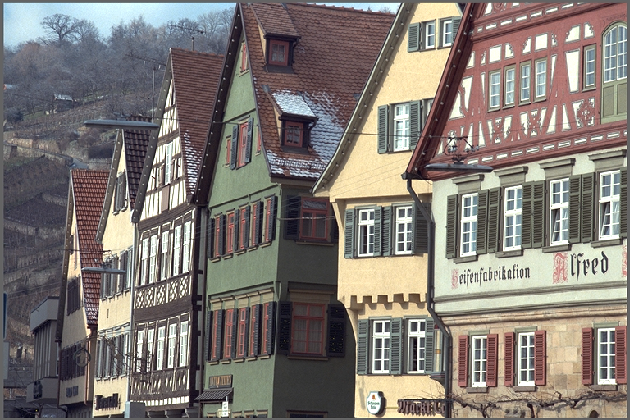
\includegraphics[width=\textwidth]{../img/liveref66.pdf}
    \legend{Fonte: \cite{livedb}}
  \end{minipage}
  \hfill
  \begin{minipage}{0.48\textwidth}
    \centering
    \caption{Imagem distorcida LIVE} \label{fig:livedist}
    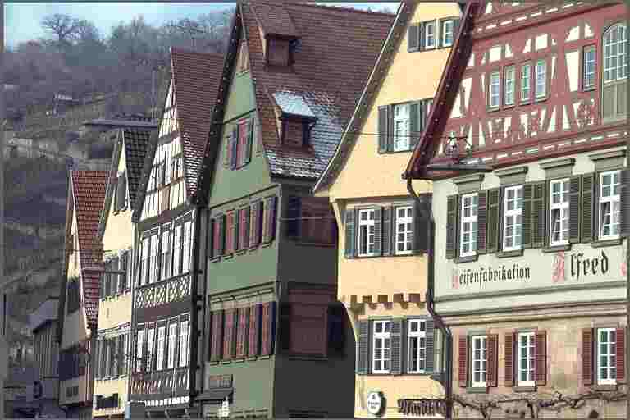
\includegraphics[width=\textwidth]{../img/liveref90.pdf}
    \legend{Fonte: \cite{livedb}}
  \end{minipage}
\end{figure}

Segundo a LIVE, o estudo que gerou as bases conduziu duas sessões de avaliação distintas. Os pesquisadores tiveram o cuidado de apresentar, em ambas as sessões, todas as imagens de referência e suas respectivas distorções. A quantidade de sujeitos no experimento foi diferente em cada sessão: na primeira, houve vinte sujeitos; apenas treze na segunda. Os pesquisadores afirmam que a escolha das imagens para o estudo foi tal que possibilitaria uma distribuição aproximadamente uniforme das notas de avaliação, o que pode ser visualizado no histograma da \autoref{graf:liveHist}, gerado diretamente a partir dos valores das notas individuais (OS). Não foi imposta restrição de distância de visualização para a avaliação e as imagens foram mostradas aos sujeitos aleatoriamente. Para emitir suas opiniões, os sujeitos poderiam levar o tempo que necessitassem, mas poderiam visualizar cada imagem apenas uma vez. Os pesquisadores promoveram uma pequena sessão de treinamento antes do início de cada sessão de avaliação. Estas informações e maiores detalhes podem ser obtidos no \emph{site} da referida base.\cite{livedb}

\begin{figure}[htb]
%	\label{graf:liveHist}
	\centering
	\begin{minipage}{.8\textwidth}
		\caption{Histograma de avaliação subjetiva  --- LIVE}\label{graf:liveHist}
		\centerline{\includegraphics{../../graphs/L_Hist_OSs.pdf}}
	\legend{Histograma gerado a partir dos OS sobre a totalidade das imagens da base}
	\end{minipage}
\end{figure}

\begin{figure}[htb]
 \label{fig:toyaex}
 \centering
  \begin{minipage}{0.48\textwidth}
    \centering
    \caption{Imagem de referência Toyama} \label{fig:toyaref}
    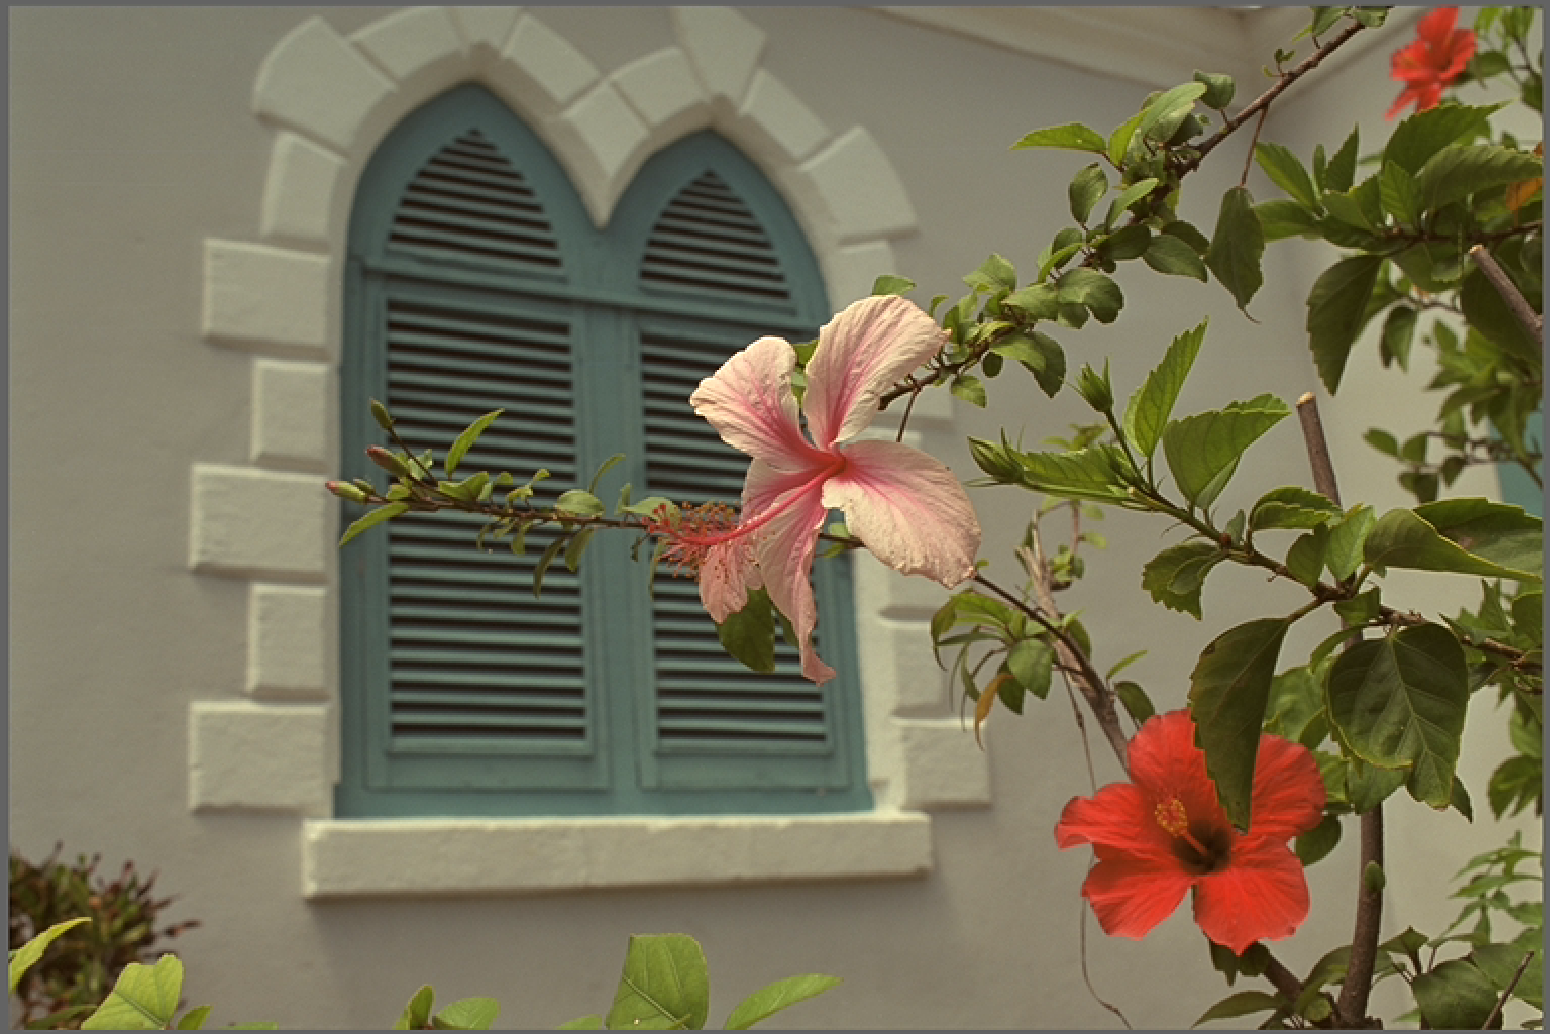
\includegraphics[width=\textwidth]{../img/toyaref07.pdf}
    \legend{Fonte: \cite{Tourancheau2008}}
  \end{minipage}
  \hfill
  \begin{minipage}{0.48\textwidth}
    \centering
    \caption{Imagem distorcida Toyama} \label{fig:toyadist}
    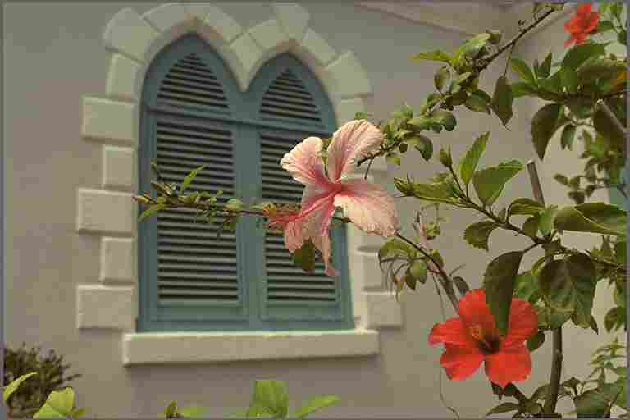
\includegraphics[width=\textwidth]{../img/toyadist07_79.pdf}
    \legend{Fonte: \cite{Tourancheau2008}}
  \end{minipage}
\end{figure}

Segundo o arquivo de informações que acompanha a base Toyama, foram dezesseis não-peritos que avaliaram as imagens dessa base, em sua maioria estudantes, não informando se houve ou não sessões distintas (e por isso assumimos uma única sessão). Da mesma forma que a LIVE, as imagens foram apresentadas aleatoriamente, sem restrição de tempo e também com apenas uma oportunidade de visualização para avaliação de cada imagem. Neste estudo foi imposta a distância de observação igual a quatro vezes a altura da imagem. A Toyama apresenta dezesseis valores de OS para cada imagem, totalizando, portanto, os dezesseis sujeitos no experimento. O histograma das notas de avaliação das imagens dessa base pode ser observado na \autoref{graf:toyaHist} (também gerado a partir dos OS).
 

\begin{figure}[htb]
%	\label{graf:liveHist}
	\centering
	\begin{minipage}{.8\textwidth}
		\caption{Histograma de avaliação subjetiva --- Toyama}\label{graf:toyaHist}
		\centerline{\includegraphics{../../graphs/T_Hist_OSs.pdf}}
		\legend{Histograma gerado a partir dos OS sobre a totalidade das imagens da base}
	\end{minipage}
\end{figure}

Ambos os grupos de pesquisa deram a seus sujeitos uma escala qualitativa conforme o exposto na \autoref{tab:avQual} mas cada uma associou a essas palavras uma escala quantitativa diferente. Além de os intervalos de avaliação serem distintos, como pode ser observado na \autoref{tab:bds}, outra diferença se faz digna de nota: a LIVE considera contínuo e linear o domínio de avaliação, enquanto a Toyama considera esse domínio discreto. Ou seja, na LIVE encontraremos notas como $4,55$, ou $94,2$ e na Toyama, apenas os inteiros no intervalo $[1,5]$. A Toyama ainda informa que seus testes foram executados conforme as condições de avaliação apontadas no ITU-R Rec. 500-10 (de março de 2010). 

\section{Considerações Estatísticas}

Comentaremos sobre a nossa interpretação dos dados e as ferramentas utilizadas para chegar a conclusões sobre esses dados.

\subsection{Níveis de Medição}

Existem quatro tipos de medição, cujos nomes podem se referir aos dados que resultam de tais medições, que indicam o tipo de dado com que se trabalha \cite[p.02-04]{boslaugh2008}:

\begin{description}
	\item{\textbf{Dados Racionais:}} A maioria das medições físicas. Os dados desse tipo de medição são naturalmente ordenáveis (têm uma ordem clara), os intervalos que distanciam duas unidades de medição são constantes; e esses dados tem um zero natural. Um exemplo: ao medir-se o comprimento de uma pessoa, faz sentido dizer que um adulto de $1,80m$ é duas vezes maior que uma criança de $0,90m$. Faz sentido também que se meça $0,0m$, e os dados $0,90m$ $0,20m$, $1,20m$ podem ser ordenados de forma crescente. Esse tipo de dado é chamado racional por ser pertinente a operação de divisão (razão) entre dois de seus elementos: a relação entre as alturas $1,8/0,9$ é $2$.
	\item{\textbf{Dados Intervalares:}} Possuem as mesmas características dos dados racionais, com a excessão do zero natural, o que faz com que a razão entre dois elementos de um conjunto de dados intervalares seja sem significado. Um exemplo é a escala Celsius, utilizada para medir temperatura. Ainda que a distância entre $10\,^{\circ}\mathrm{C}$ e $11\,^{\circ}\mathrm{C}$ seja igual a distância entre $20\,^{\circ}\mathrm{C}$ e $21\,^{\circ}\mathrm{C}$, não faz sentido dizer que $20\,^{\circ}\mathrm{C}$ é duas vezes mais quente do que $10\,^{\circ}\mathrm{C}$, já que a razão (e sua contra-partida, a multiplicação) não é definida para esse tipo de dado.
	\item{\textbf{Dados Ordinais:}} Possuem uma ordem natural, no sentido de que valores mais altos representam mais de uma determinada característica do que valores menores. Não existe analogia métrica, onde se possa colocar uma régua e medir a distância entre dois de seus pontos, apesar de eles poderem ser, claramente, ordenados do mais ao menos significativo, por exemplo. É o caso, por exemplo, do nível de adequação de candidatos a vagas de emprego. Sempre haverá um mais apto e um menos apto, não se pode, contudo, medir a distância entre eles. Operações como adição e subtração perdem significado aqui, já que não dá para se dizer quanto de ``aptidão'' tem-se que adicionar a um currículo A para que ele tenha a mesma ``aptidão'' à vaga que um currículo B. Esses são dados essecialmente categóricos e ferramentas como a média não têm sentido aqui; ao invés da média tem-se que adotar a mediana como indicador de centralidade.
	\item{\textbf{Dados Nominais:}} Aqui, números (quando usados) não trazem informação de ordenação, já que esses dados não apresentam características que os permitam ser ordenados. É o caso, por exemplo, da classificação por gênero: existem apenas dois, distintos, sem informações de ordem, masculino e feminino. Para o caso em que ambas as classes fossem representadas por números, esses números não teriam significado de grandeza (1 para feminino e 0 para masculino, por exemplo), serviriam apenas para facilitar a arrecadação dos dados ou sua posterior organização por um sistema computadorizado. Aqui, da mesma forma, não fazem sentido as operações aritméticas e ferramentas categóricas têm que ser usadas para tratar esse tipo de dado.
\end{description}

Note que a classificação acima não leva em consideração se os dados são discretos ou contínuos. Dados contínuos são aqueles que podem assumir qualquer valor, ou qualquer valor dentro de um intervalo limitado (como é o caso da escala utilizada pela LIVE); dados discretos podem assumir apenas valores exatos e têm suas fronteiras bem delimitadas (como é o caso das medições produzidas pela Toyama). Outro exemplo de dados discretos são aqueles que advém de contagem, como o número de crianças em uma residência.

Assim, a partir do exposto, dados intervalares e racionais podem ser contínuos, enquanto os ordinais e nominais tendem a ser discretos. Por outro lado, não existe uma barreira intransponível entre os dois tipos de dados: ao se registrar a idade de indivíduos em anos está-se discretizando uma entidade contínua. Outro exemplo é a categorização de dados contínuos para melhor manipulação ou exibição dos dados, como se faz ao se gerar um histograma.

À luz do exposto, alguns detalhes sobre as bases e os processos de arrecadação de dados pelos laboratórios que ora consideramos ficam mais claros.

É fácil perceber que a quantidade de ``excelência'' de uma imagem não pode ser quantificada, já que avaliações por adjetivos não são matematicamente operacionalizadas diretamente (dois ``regulares'' não fazem um ``bom''), e ferramentas estatísticas que lidam com categorias seriam mais adequadamente utilizadas. Nesse quesito, equívocos são cometidos ao misturarem-se dois domínios de dados para análise estatística, e esses equívocos advém da própria organização que padroniza essa coleta de dados (ITU).

 % Considerações Iniciais

% Aqui é descrita toda a teoria necessária para o entendimento do trabalho. É um capítulo de caráter informativo e não deve ser grande em demasia.
% É um capítulo generalista, onde se fala sobre os principais conceitos da área
% Sub-dividido em:
%  Introdução
%  Desenvolvimento
%  Conclusão
%

\chapter{Procedimento Tradicional}

Os procedimentos de validação de uma métrica de qualidade visual passam por três testes, de acordo com as recomendações do ITU~\cite{itut2004}:

\begin{enumerate}
	\item Precisão;
	\item Monotonicidade;
	\item Consistência.
\end{enumerate}


 % Análise Comparativa

% Este é um capítudo de revisão de literatura
% Sub-dividido em:
%  Introdução: apresentada a lógica do capítulo e o que será encontrado em cada uma das seções.
%  Desenvolvimento:
%	Qual o problema analisado no trabalho?
%	Por que ele é importante?
%	O que se tem feito no mundo para resolvê-lo?
%	O ideal é se ter um estudo qeu disserte/comente os trabalhos citados, mostrando a sua relação com o problema, as vantagens e desvantagens de cada trabalho
%		citado.
%	Qual a contribuição desse trabalho? É o diferencial da proposta, principalmente, em relação às referências citadas na revisão bibliográfica.
%  Conclusão: faça referência aos pontos importantes do capítulo, que podem ser transversais às seções. Estes pontos serão, muito provavelmente, úteis ao leitor
% 		dos capítulos seguintes. Tente sempre conectar os capítulos textualmente, com 'ganchos' para o próximo assunto.
%
% Este capítulo deve omitir a teoria básica, apresentada no capítulo anterior.
% Sendo uma revisão de literatura, deve apresentar soluções dos diversos autores para o problema apresentado (ou seja, diante do problema exposto, o que tem sido feito 
% para resolvê-lo? Como? Por quem?
% Destaque como a literatura resolve o problema, vantagens e desvantagens.
%
% Este capítulo deve ser finalizado com a indicação da contribuição do trabalho e indicar o diferencial em relação as abordadas no capítulo. Maiores detalhes sobre a
% proposta do trabalho serão apresentados no próximo capítulo.

\include{cap03} 

% Esse capítulo aborda a contribuição do trabalho. Se houver necessidade, pode-se incluir uma seção para se destacar 'uma teoria nova' (ou não citada no capítulo anterior)
% e que seja importante para o entendimento da contribuição.
%
% Sub-dividido em:
%  Introdução
%  Desenvolvimento
%  Conclusão 

% \chapter{Descrição do Cenário ou ambiente usado para a obtenção dos resultados. E resultados.}

% Aborda todos os procedimentos utilizados para a obtenção dos resultados.
% Se o trabalho for uma simulação, apresentar o cenário de simulação utilizado.
% Se for um trabalho prático, deve-se descrever o setup laboratorial juntamente com as arquiteturas eletrônicas usadas.
% A metodologia utilizada para validar os resultados/contribuições. Experiências realizadas devem ser descritas aqui.
%   Quais foram os experimentos realizados para se chegar nos resultados?
%   Como esses resultados foram validados?
% Os resultados apresentados devem ser apresentados e analisados! Analise resultados, não descreva gráficos.
% Importante é subsidiar o leitor com todas as informações usadas para a obtenção dos resultados (parâmetros devem ser especificados, quando possível, anexar as listagens
% dos resultados.
%
% Sub-dividido em:
%  Introdução
%  Desenvolvimento
%  Conclusão 
%  
\include{cap04}
\include{concl}

% Revisão do trabalho desenvolvido
%   Objetivos do trabalho, conclusões relevantes
% Resultados / contribuições relevantes
% Resultado 1
%   Caracterização do resultado. Justificativa
%   Aspectos positivos e negativos.
% Resultado 2
% Resultado 3
% Fundamental na conclusão: TRABALHOS FUTUROS, identificar novos trabalhos que possam ser desenvolvidos sobre os resultados encontrados; fornecendo, sempre que possível, 
% 	informações e subsídios de como se pode progredir. Tente evitar esboçar uma lista de possibilidades de trabalhos futuros sem indicar como esses podem ser viabilizados
% 	a partir dos resultados encontrados.
% 
% Referências Bibliográficas: em se tratando de Ref. Bib., todas devem estar citadas no texto e listadas de acordo com a ordem de citação! Comumente adota-se o padrão de citação
% de artigos como os do IEEE

\bibliography{references}
%\bibliographystyle{bnt-num}


\end{document}

